%%%%%%%%%%%%%%%%%%%%%%%%%%%%%%%%%%%%%%%%%
% Short Sectioned Assignment
% LaTeX Template
% Version 1.0 (5/5/12)
%
% This template has been downloaded from:
% http://www.LaTeXTemplates.com
%
% Original author:
% Frits Wenneker (http://www.howtotex.com)
%
% License:
% CC BY-NC-SA 3.0 (http://creativecommons.org/licenses/by-nc-sa/3.0/)
%
%%%%%%%%%%%%%%%%%%%%%%%%%%%%%%%%%%%%%%%%%

%----------------------------------------------------------------------------------------
%	PACKAGES AND OTHER DOCUMENT CONFIGURATIONS
%----------------------------------------------------------------------------------------

\documentclass[paper=a4, fontsize=11pt]{scrartcl} % A4 paper and 11pt font size

\usepackage[T1]{fontenc} % Use 8-bit encoding that has 256 glyphs
\usepackage{fourier} % Use the Adobe Utopia font for the document - comment this line to return to the LaTeX default
\usepackage[english]{babel} % English language/hyphenation
\usepackage{amsmath,amsfonts,amsthm} % Math packages
\usepackage{cancel}
\usepackage{graphicx}

\usepackage{lipsum} % Used for inserting dummy 'Lorem ipsum' text into the template

\usepackage{sectsty} % Allows customizing section commands
\allsectionsfont{\centering \normalfont\scshape} % Make all sections centered, the default font and small caps

\usepackage{svg}

\usepackage{siunitx}
\sisetup{detect-all}

\usepackage{fancyhdr} % Custom headers and footers
\pagestyle{fancyplain} % Makes all pages in the document conform to the custom headers and footers
\fancyhead{} % No page header - if you want one, create it in the same way as the footers below
\fancyfoot[L]{} % Empty left footer
\fancyfoot[C]{} % Empty center footer
\fancyfoot[R]{\thepage} % Page numbering for right footer
\renewcommand{\headrulewidth}{0pt} % Remove header underlines
\renewcommand{\footrulewidth}{0pt} % Remove footer underlines
\setlength{\headheight}{13.6pt} % Customize the height of the header

\numberwithin{equation}{section} % Number equations within sections (i.e. 1.1, 1.2, 2.1, 2.2 instead of 1, 2, 3, 4)
\numberwithin{figure}{section} % Number figures within sections (i.e. 1.1, 1.2, 2.1, 2.2 instead of 1, 2, 3, 4)
\numberwithin{table}{section} % Number tables within sections (i.e. 1.1, 1.2, 2.1, 2.2 instead of 1, 2, 3, 4)

\setlength\parindent{0pt} % Removes all indentation from paragraphs - comment this line for an assignment with lots of text

%----------------------------------------------------------------------------------------
%	TITLE SECTION
%----------------------------------------------------------------------------------------

\newcommand{\horrule}[1]{\rule{\linewidth}{#1}} % Create horizontal rule command with 1 argument of height

\title{
\normalfont \normalsize 
\horrule{0.5pt} \\[0.4cm] % Thin tp horizontal rule
\huge Solving the differential equation of a falling raindrop with air resistance\\ % The assignment title
\horrule{2pt} \\[0.5cm] % Thick bottom horizontal rule
}

\author{Tobias Kuhn} % Name

\date{\normalsize\today} % Today's date or a custom date

\begin{document}

\maketitle % Print the title

\section{What are we trying to do here?}

We want to spend some time thinking about raindrops and air resistance. 
In particular, we want to find a function $v_y(t)$ which maps time $t$ to the velocity 
of a falling raindrop. \vspace{\baselineskip}

We assume that our mathematical raindrop has both a constant mass and a fixed shape.
Furthermore, we assume that there is no wind and the only forces governing the raindrops movement are 
$F_g$ (gravitational pull) and $F_r$ (air resistance).
\begin{align} \label{eq:1}
F_{tot} &= F_g - F_r
\end{align}
The air resistance in our model is proportional to $v_y(t)^2$.\footnote{Quadratic drag models the air resistance sensibly at 
high velocities (i.e. high Reynolds number, Re > ~1000). Our raindrop has a Re of about 3000.} We also introduce air resistance coefficient $k$ 
which allows us to adjust our air resistance curve to be as close as possible to the real air resistance a falling drop would experience
at fairly high velocities.
\begin{align} \label{eq:2}
F_r &= k \cdot v_y(t)^2
\end{align}
But what is a good value for $k$? Seeking for a fitting coefficient $k$, we stumble upon a 1969 paper 
by G. B. Foote and P. S. Du Toit titled \textit{Terminal Velocity of Raindrops Aloft}.
\footnote{ https://journals.ametsoc.org/doi/pdf/10.1175/1520-0450\%281969\%29008\%3C0249\%3ATVORA\%3E2.0.CO\%3B2 }
\vspace{\baselineskip}

Armed with this paper, we go through a few steps which conclude in a value for our air resistance coefficient $k$.
First, we use figure 2 on page 251 to determine the terminal velocity $V$ of a raindrop with a diameter of $5[\si{\milli\meter}]$
at an atmospheric pressure of $1013[\si{\milli\bar}]$ and get 
\begin{align} \label{eq:2.5}
V &= 9.1[\si{\meter\per\second}].
\end{align}
Next we use the terminal velocity $V$, the radius $r$ and the kinematic viscosity of the air $\nu$ to calculate Reynolds number $R_e$.
\begin{align} \label{eq:3}
R_e &= \frac{2rV}{\nu} \\
    &= \frac{2 \cdot 0.0025[\si{\meter}] \cdot 9.1 [\si{\meter\per\second}]}{1.516 \cdot 10^{-5}[\si{\meter\squared\per\second}]} \\
    &= 3001.0
\end{align}
Now that we've got Reynolds number for our specific raindrop, we are able to get drag coefficient $C_D$ by consulting figure 1
on page 250. We get a value of 0.645. Armed with the drag coefficient $C_D$, radius $r$ and air density 
$\rho$, we are finally able to calculate the magnitude of air resistance coefficient $k$ using equation (1) on page 249.
\begin{align} \label{eq:4}
k &= \frac{1}{2} \rho C_D \pi r^2 \\
  &= \frac{1}{2} \cdot 1.225 [\si{\kilogram\per\meter\cubed}] \cdot 0.645 \cdot \pi \cdot 6.25 \cdot 10^{-6} [\si{\meter\squared}] \\
  &=  7.757 \cdot 10^{-6}[\si{\kilogram\per\meter}]
\end{align}
Note how the air resistance coefficient $k$ comes with the SI units [\si{\kilogram\per\meter}].
When using $k$ in (\ref{eq:2}) we expect the resulting SI units to be [\si{\kilogram\meter\per\second\squared}].
\begin{align} \label{eq:5}
F_r &= k \cdot v_y(t)^2 \\
[\si{\kilogram\meter\per\second\squared}]  &= [\si{\kilogram\per\meter}] \cdot [\si{\meter\squared\per\second\squared}] \\
  &= [\si{\kilogram\meter\per\second\squared}]
\end{align}
And indeed, [\si{\kilogram\meter\per\second\squared}] is what we get.

\section{the equation of motion}
Now we are finally ready to construct and solve the differential equation of our raindrop model.
We start by taking a closer look at equation (\ref{eq:1}). Here it is again:
\begin{align}
F_{tot} &= F_g - F_r. \tag{\ref{eq:1}}
\end{align}
Adding all the Forces working on our raindrop yields $F_{tot}$. And since $F_{tot}$ accounts for all the forces, we can use it to
calculate the resulting acceleration by inserting the famous 
\begin{align} \label{eq:6}
F &= m \cdot a_y(t).
\end{align}
Doing this, we get
\begin{align} \label{eq:7}
m \cdot a_y(t) &= F_g - F_r. 
\end{align}
Next we insert the following two equations 
\begin{align}
F_g &= m \cdot g \label{eq:8} \\
F_r &= k \cdot v_y(t)^2 \tag{\ref{eq:2}}
\end{align}
($g$ being the acceleration of gravity) into (\ref{eq:7}) and get
\begin{align} \label{eq:9}
m \cdot a_y(t) &= m \cdot g - k \cdot v_y(t)^2. 
\end{align}
And finally, we rewrite $a_y(t)$ as the derivative of $v_y(t)$ and arrive at
\begin{align} \label{eq:10}
m \cdot \frac{d}{dt} v_y(t) &= m \cdot g - k \cdot v_y(t)^2. 
\end{align}
Now we got the newtonian equation of motion for our raindrop. We want to find a specific function $v_y(t)$ which, 
when plugged into this equation satisfies it at any value t.
\section{Solving the differential equation}
We start by tidying up (\ref{eq:10}) by dividing both sides of the equation by $m$
\begin{align} \label{eq:11}
\frac{d}{dt} v_y(t) &= g - \frac{k}{m} \cdot v_y(t)^2
\end{align}
Next we get everything ready for the first ingenious math technique by isolating $g$
\begin{align} \label{eq:12}
\frac{d}{dt} v_y(t) &= g \left(1 - \frac{k}{gm} \cdot v_y(t)^2\right)
\end{align}
and introducing $\beta$ as a placeholder variable to get rid of some of the clutter:
\begin{align} \label{eq:13}
\beta^2 &= \frac{k}{gm}
\end{align}
this placeholder variable enables us to rewrite (\ref{eq:12}) as

\begin{align} \label{eq:13.1}
\frac{d}{dt} v_y &= g \left(1 - \beta^2 v_y^2\right) \\
                    &= g \left(1^2 - (\beta v_y)^2\right) \\
                    &= g \left((1 - \beta v_y)\cdot (1 + \beta v_y)\right)
\end{align}
Starting at (\ref{eq:13.1}) we are shortening $v_y(t)$ to $v_y$ to make the equations easier to read. Now we divide both sides of the equation by the expression in the brackets. This yields
\begin{align} \label{eq:13.2}
\frac{1}{(1 - \beta v_y)\cdot (1 + \beta v_y)} \cdot \frac{d v_y}{dt}  &= g.
\end{align}
Next we switch around the terms to make the equation a bit more pleasant to look at.
\begin{align} \label{eq:14}
g  &= \frac{1}{(1 - \beta v_y)\cdot (1 + \beta v_y)} \cdot \frac{d v_y}{dt}
\end{align}
We take the integral with respect to t on both sides of the equation.
\begin{align} \label{eq:15}
\int g \cdot dt &= \int \frac{1}{(1 - \beta v_y)\cdot (1 + \beta v_y)} \cdot \frac{d v_y}{dt} \cdot dt
\end{align}
The left side of the equation becomes $g \cdot t + C_1$. $C_1$ being the constant of integration.
But what about the right side?
\begin{align} 
g \cdot t + C_1 &= \int \frac{1}{(1 - \beta v_y)\cdot (1 + \beta v_y)} \cdot \frac{d v_y}{\cancel{dt}} \cdot \cancel{dt} \label{eq:16}\\
                &= \int \frac{1}{(1 - \beta v_y)\cdot (1 + \beta v_y)} \cdot d v_y \label{eq:17}
\end{align}
The two $dt$ terms cancel out leaving us with with an integral with respect to $dv_y$.
The cancellation of the two $dt$ terms is the first ingenious math technique used on the journey to the solution of this differential equation.
\vspace{\baselineskip}

But we still need to actually solve the integral on the right side. What holds us back is the squared $v_y$, which emerges as soon as we
multiply out all the terms in the denominator. But why did we rearrange the terms in the denominator anyway? This is because we are about to
use partial-fraction decomposition on it. We want to concentrate on the partial-fraction decomposition, so let's 
forget about the integral and let $p$ be the fraction inside the integral of equation (\ref{eq:17}).
\begin{align} \label{eq:18}
p &= \frac{1}{(1 - \beta v_y)\cdot (1 + \beta v_y)}
\end{align}
Let's examine the nominator. It is 1. What if we defined the following equation?
\begin{align} \label{eq:19}
1 &= A \cdot (1 - \beta v_y) + B \cdot (1 + \beta v_y)
\end{align}
Equation (\ref{eq:19}) also evaluates to 1, so clearly we are able to insert it in the nominator of equation (\ref{eq:18})
which gives us
\begin{align} 
p &= \frac{A \cdot (1 - \beta v_y) + B \cdot (1 + \beta v_y)}{(1 - \beta v_y)\cdot (1 + \beta v_y)} \\
  &= \frac{A \cdot \cancel{(1 - \beta v_y)}}{\cancel{(1 - \beta v_y)}\cdot (1 + \beta v_y)} +
     \frac{B \cdot \cancel{(1 + \beta v_y)}}{(1 - \beta v_y)\cdot \cancel{(1 + \beta v_y)}} \\
  &= \frac{A}{1 + \beta v_y} + \frac{B}{1 - \beta v_y} \label{eq:20}
\end{align}

The resulting equation (\ref{eq:20}) will allow us to finally compute the integral in (\ref{eq:17}). The only thing left to do is to get
specific values for A and B. Clearly, equation (\ref{eq:19}) doesn't hold true for any value $A$ and $B$. But what are the values which, when
inserted, keep (\ref{eq:19}) satisfied no matter what magnitude $v_y(t)$ takes on? Since equation (\ref{eq:19}) has to hold true
for any value a generic function $v_y(t)$ might return, it also has to hold true for the following two cases:
\begin{align}
v_y(t) &= \frac{1}{\beta}  \label{eq:21} \\
v_y(t) &= - \frac{1}{\beta} \label{eq:22}
\end{align}
Inserting (\ref{eq:21}) into (\ref{eq:19}) yields
\begin{align} 
1 &= A \left(1 - \beta \cdot \frac{1}{\beta}\right) + B \left(1 + \beta \cdot \frac{1}{\beta}\right) \\
  &= A \left(1 - \cancel{\beta} \cdot \frac{1}{\cancel{\beta}}\right) + B \left(1 + \cancel{\beta} \cdot \frac{1}{\cancel{\beta}}\right) \\
  &= A (1 - 1) + B (1 + 1) \\
  &= A 0 + B 2 \\
  &= 2B. \label{eq:23}
\end{align}
From (\ref{eq:23}) we conclude that
\begin{align}
B &= \frac{1}{2}.  \label{eq:24}
\end{align}
Likewise, inserting (\ref{eq:22}) into (\ref{eq:19}) yields
\begin{align} 
1 &= A \left(1 - \beta \cdot -\frac{1}{\beta}\right) + B \left(1 + \beta \cdot -\frac{1}{\beta}\right) \\
  &= A \left(1 + \beta \cdot \frac{1}{\beta}\right) + B \left(1 - \beta \cdot \frac{1}{\beta}\right) \\
  &= A \left(1 + \cancel{\beta} \cdot \frac{1}{\cancel{\beta}}\right) + B \left(1 - \cancel{\beta} \cdot \frac{1}{\cancel{\beta}}\right) \\
  &= A (1 + 1) + B (1 - 1) \\
  &= A 2 + B 0 \\
  &= 2A. \label{eq:25}
\end{align}
From (\ref{eq:25}) we conclude that
\begin{align}
A &= \frac{1}{2}.  \label{eq:24}
\end{align}
We insert above results for $A$ and $B$ into equation (\ref{eq:20}) and get
\begin{align}
  p &= \frac{1}{2}\left(\frac{1}{1 + \beta v_y} + \frac{1}{1 - \beta v_y}\right). \label{eq:25}
\end{align}
Let's put $p$ back into \ref{eq:17} and finally calculate the integral.
\begin{align} 
g t + C_1  &= \frac{1}{2} \int \left(\frac{1}{1 + \beta v_y} + \frac{1}{1 - \beta v_y}\right) d v_y  \\
2g t + C_2 &= \int \left(\frac{1}{1 + \beta v_y} + \frac{1}{1 - \beta v_y}\right) d v_y \\
           &= \int (1 + \beta v_y)^{-1} d v_y + \int (1 - \beta v_y)^{-1} d v_y \\
           &=  \frac{1}{\beta} \ln{\left|1 + \beta v_y \right|} -
               \frac{1}{\beta} \ln{\left|1 - \beta v_y \right|} + C_3 \\
           &=  \frac{1}{\beta} \left( \ln{\left|1 + \beta v_y \right|} -
               \ln{\left|1 - \beta v_y \right|} \right) + C_3 \label{eq:26}
\end{align}
Because $log(a) - log(b) = log(\frac{a}{b})$, we can rewrite (\ref{eq:26}) as
\begin{align} 
2g t + C_4 &=  \frac{1}{\beta} \ln{\left|\frac{1 + \beta v_y}{1 - \beta v_y} \right|} \label{eq:27}
\end{align}
We are taking the absolute value of the expression inside the natural logarithm because logarithms only work with
positive numbers. If we are able to show that $1 - \beta v_y \geq 0$ over the complete range of $v_y(t)$ we can
get rid of the absolute value signs since we are certain that the expression will be positive.

To examine the Range of $v_y(t)$,
we first acknowledge the fact that $|F_g| \geq |F_r|$ will always be true and thus the velocity will always be positive 
(we have setup the equation of motion in such a way that positive means downwards/towards the earth.) Therefore, $v_y(t) \geq 0$ over the 
complete domain $0 \leq t \leq \infty$. From (\ref{eq:2.5}) we also know that terminal velocity $V = 9.1[\si{\meter\per\second}]$.
Thus, the Range of $v_y(t)$ is 
\begin{equation} 
0 \leq v_y(t) \leq 9.1[\si{\meter\per\second}].
\end{equation}
But what about $\beta$? In (\ref{eq:13}) we defined $\beta$ as follows:
\begin{align} \label{eq:13.1}
\beta^2 &= \frac{k}{gm}
\end{align}
Therefore,
\begin{align} \label{eq:28}
\beta &= \sqrt{\frac{k}{gm}}.
\end{align}
We know the $k$ and $g$, and from yet another raindrop related paper
\footnote{Humphreys, W. J. Physics of the Air. New York: Dover, 1964: 279} we know that our raindrop, which we decided to have a diameter of
$d = 5 [\si{\milli\meter}]$, has a mass $m = 70 [\si{\milli\gram}]$.
It follows then, that
\begin{align} 
\beta &= \sqrt{\frac{k}{gm}}. \\
      &= \sqrt{\frac{7.757 \cdot 10^{-6}[\si{\kilogram\per\meter}]}{9.81 [\si{\meter\per\second\squared}] \cdot 7 \cdot 10^{-5} [\si{\kilo\gram}]}} \\
      &= 0.106 [\si{\per\meter\second}]. \label{eq:29}
\end{align}
Using terminal velocity $V$ and the calculated value for $\beta$, we calculate the maximum value $\beta v_y$ is able to take as follows 
\begin{align} 
\beta V &= 0.106 [\si{\per\meter\second}] \cdot 9.1[\si{\meter\per\second}] \\
        &= 0.9646 .\label{eq:30}
\end{align}
Because of (\ref{eq:30}), we know that $1 - \beta v_y \geq 0$ holds true over the complete range of $v_y(t)$. And thus we are able to
get rid of the absolute value signs in (\ref{eq:27}), arriving at
\begin{align} 
2g t + C_4 &=  \frac{1}{\beta} \ln{\left(\frac{1 + \beta v_y}{1 - \beta v_y} \right)} \label{eq:31}
\end{align}
This is a good time to decide what to do with differential constant $C_4$. $C_4$s physical meaning is equivalent 
to that of the start velocity of our model at $t = 0$. We want the raindrop to start at $v_y(t_0) = 0 [\si{\meter\per\second}]$.
Therefore, we set it to 0.
\begin{align} 
2 g \beta t &=  \ln{\left(\frac{1 + \beta v_y}{1 - \beta v_y} \right)} \label{eq:32}
\end{align}
So far so good. But how are we supposed to solve [\ref{eq:32}] for $v_y$? Yet another ingenious math strategy is about to unfold.
Let's recall the very basic concept of what a logarithm is:
\begin{align} 
3 &=  \log_{10}{(1000)} \label{eq:33}
\end{align}
Question: To what power do I raise 10 to get 1000?

Answer: 3.
\vspace{\baselineskip}

That's what algorithms are all about. And it is easy to see how we are able to rearrange the variables in (\ref{eq:33})
to get
\begin{align} 
10^3 &=  1000 \label{eq:34}
\end{align}
Applying the same rearrangement operation to (\ref{eq:32}) yields
\begin{align} 
e^{2 g \beta t} &=  \frac{1 + \beta v_y}{1 - \beta v_y}. \label{eq:35}
\end{align}
We're almost there. Some more variable shuffling 
\begin{align} 
e^{2 g \beta t} &=  \frac{1 + \beta v_y}{1 - \beta v_y} \\
e^{2 g \beta t} \cdot \left(1 - \beta v_y \right) &= 1 + \beta v_y  \\
e^{2 g \beta t} - e^{2 g \beta t}\beta v_y &= 1 + \beta v_y  \\
e^{2 g \beta t} - 1 &= \beta v_y (1 + e^{2 g \beta t})
\end{align}
and we arrive at the final solution
\begin{align}
v_y(t) &= \frac{1}{\beta} \cdot \frac{e^{2 g \beta t} - 1}{e^{2 g \beta t} + 1}.\label{eq:36}
\end{align}
The graph below shows $v_y(t)$ plotted over the range $0[\si{\second}] \leq t \leq 10[\si{\second}]$.

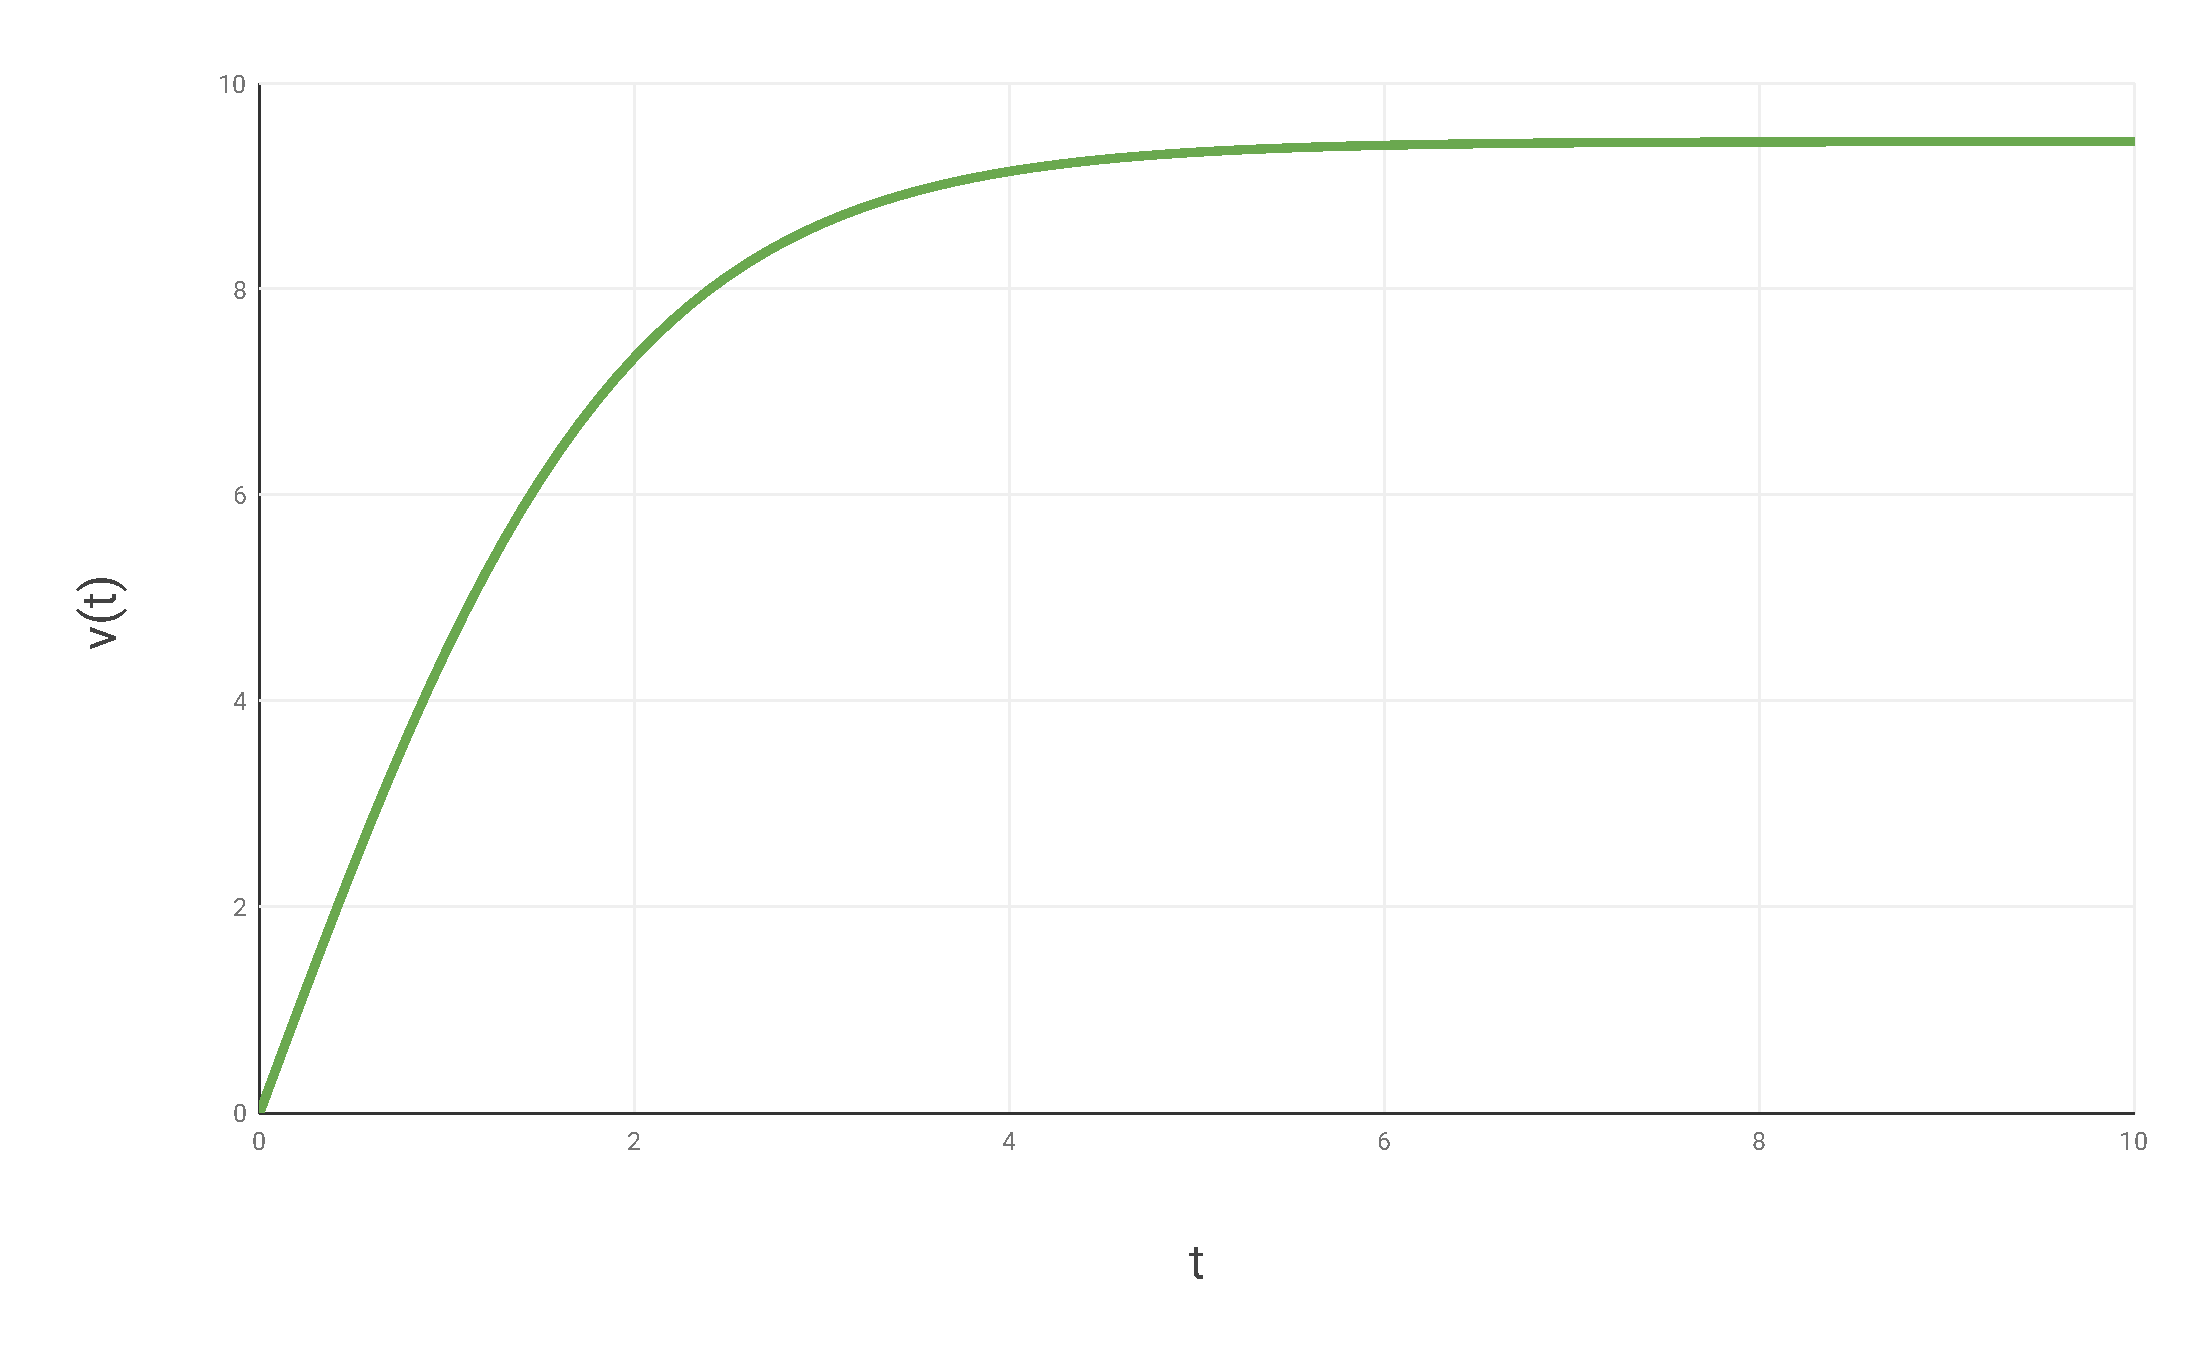
\includegraphics[width=.95\linewidth]{graph}

It seems like $v_y(t)$ is converging to some value. This confirms our intuition about falling objects.
The value $v_y(t)$ is converging to, of course, is the terminal Velocity.
We already know the terminal Velocity $V$ from equation (\ref{eq:2.5}). But this $V$ isn't very mathematical. 
We got it from a graph on a paper about the terminal velocities of raindrops.
We needed it to get a sensible drag coefficient $C_d$, but in order to know the true 
mathematically correct terminal velocity (let's call it $V_t$), we need to calculate the limit 
of $v_y(t)$ as $t$ approaches infinity.
\begin{align} 
lim_{t\to\infty} v_y(t) &= V_t = lim_{t\to\infty} \frac{1}{\beta} \cdot \frac{e^{2 g \beta t} - 1}{e^{2 g \beta t} + 1} \label{eq:37}
\end{align}
Multiplying both the nominator and denominator of the right hand side of equation (\ref{eq:37}) by $e^{-2 g \beta t}$ we get
\begin{align} 
V_t &= lim_{t\to\infty} \frac{1}{\beta} \cdot \frac{1 - e^{-2 g \beta t}}{1 + e^{-2 g \beta t}}. \label{eq:38}
\end{align}
And since 
\begin{align} 
lim_{t\to\infty} e^{-2 g \beta t} &= 0
\end{align}
equation (\ref{eq:38}) becomes
\begin{align} 
V_t &=  \frac{1}{\beta} \cdot \frac{1 - 0}{1 + 0}. \label{eq:39} \\
    &=  \frac{1}{\beta} . \label{eq:40}
\end{align}
This turns out to be quite a surprise. The $\beta$, which we created merely as a way to keep our equations from getting too cluttered,
turns out to be the terminal Velocity $V_t$! We already calculated $\beta$ to be 0.106 [\si{\per\meter\second}] in equation (\ref{eq:29}).
Using this result to calculate $V_t$ we get
\begin{align} 
V_t &=  \frac{1}{0.106 [\si{\per\meter\second}]} \\
    &=  9.434 [\si{\meter\per\second}]
\end{align}
The units are spot on as well. Everything's falling into its place. Remember how we had to show that $1 - \beta v_y \geq 0$ is true
for the complete range of $v_y(t)$ to get rid of the absolute value signs in the equation below?
\begin{align} 
2g t + C_4 &=  \frac{1}{\beta} \ln{\left|\frac{1 + \beta v_y}{1 - \beta v_y} \right|} \tag{\ref{eq:27}}
\end{align}
We barely managed to do so in (\ref{eq:30}), but it wasn't very mathematical at all. We crudely used terminal velocity $V$ to vouch for us
that $v_y(t)$ wouldn't get too big and we are indeed able to get rid of those absolute value signs.
Armed with our new shiny $V_t = \beta^{-1}$ we can show that $1 - \beta v_y \geq 0$ holds true in a much more satisfying way:
\begin{align} 
  1 - \beta \cdot V_t &= 1 - \beta \cdot \beta^{-1} \\
  &= 0 \geq 0
\end{align}
And that's the end of our journey to solve the differential equation of a falling raindrop with air resistance proportional to the velocity squared. 

\end{document}